\chapter{Experimentos e Resultados}

\section{O Aplicativo machado}

\par
Algumas informa��es sobre o aplicativo (linguagem, n�mero de linhas, op��es de execu��o (--help), etc.
\par
Mostrar gr�fico de ortogonalidade? (m�trica x acur�cia)
\par
Mostrar tabela de acertos?
\par
O algoritmo n�o ortogonal est� quase igual ao lazy - talvez ele nem precise ser citado
\par

\begin{verbatim}
Usage: ./classifier [options]
Options:
  -i, --training-file        Set the training file
  -t, --testing-file         Set the testing file
  -s, --support              Set the support
  -c, --confidence           Set the confidence
  -r, --run-mode             Set the run mode [c,o] [CLASSICAL, ORTHOGONAL]
  -p, --pattern-set          Set the pattern set type [f,m,r] [FREQUENT, MAXIMAL,
                               RANDOM MAXIMAL]
  -n, --min-num-rules        Set the minimum number of rules
  -l, --max-num-rank-rules   Set the maximum number of rules considered in rank
                               (rank size)
  -m, --min-rule-len         Set the minimum length of the rules
  -x, --max-rule-len         Set the maximum length of the rules
  -o, --orth-mode            Set the orthogonality mode [h,p,o] [HEURISTICAL,
                               POLYNOMIAL, ORIGAMI]
  -e, --orth-metric          Set the orthogonality mode [s,c,l,a] [SIMILARITY,
                               TRANSACTION COVERAGE, CLASS COVERAGE, ALL]
  -w  --orth-method          Set the way metrics are used [s,p,a] [SET, PAIR AVERAGE,
                               ALL]
  -g  --orth-pat-ordering    Set the way patterns are ordered for orthogonality
                              heuristic [s,r,i,z,n] [SORTED, REVERSE SORTED,
                              SORTED BY SIZE, REVERSE SORTED BY SIZE, NONE]
  -a  --origami-alpha        Set the alpha parameter used by ORIGAMI
  -b  --origami-beta         Set the beta parameter used by ORIGAMI
  -d, --debug                Set the level of debug [0-4] [NODEBUG - MAXLEVEL]
  -v, --verbose              Use verbose mode
  -h, --help                 Display this information
\end{verbatim}

The figure \ref{fig:histogram_acc} shows a histogram with the best accuracies for each dataset obtained with LAC, ORIGAMI, orthogonal classifier and non-orthogonal classifier. The figure \ref{fig:histogram_pat} shows a histogram with the average number of patterns used for each classification, and the figure \ref{fig:histogram_rul} shows the average number of rules generated for each classification. For those three results it was used the best set of parameters for each dataset, for example, for anneal.ac we used support equals to 0.0001, but for waveform.ac we used support equals to  0.01, since the best results were obtained with this value.

\begin{figure}[htbp]
	\centering
	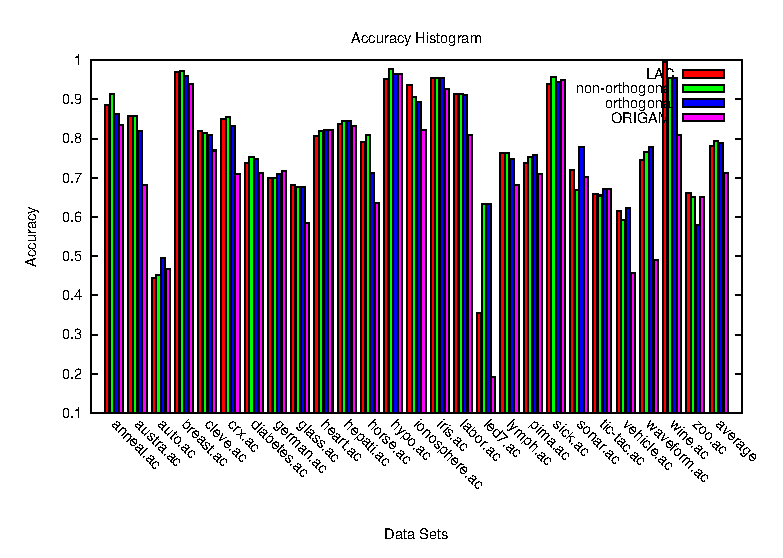
\includegraphics{graphs/histogram_acc.eps}
	\caption{Accuracy Histogram (best results for each dataset)}
	\label{fig:histogram_acc}
\end{figure}

\begin{figure}[htbp]
	\centering
	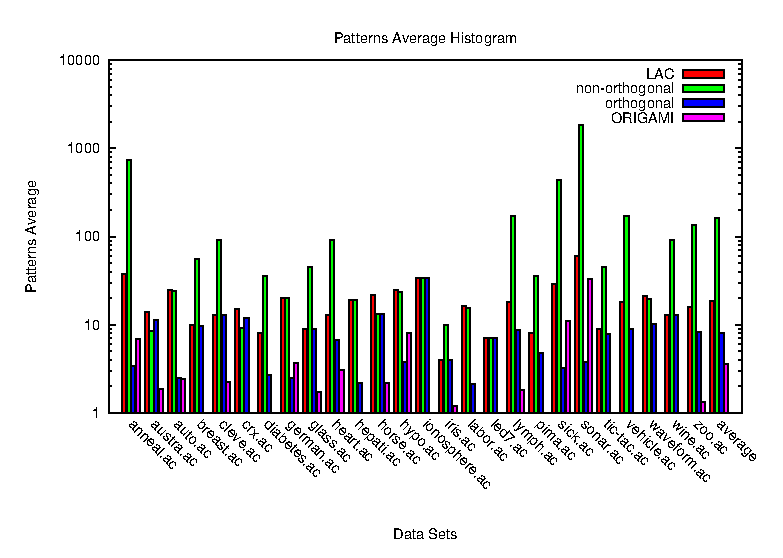
\includegraphics{graphs/histogram_pat.eps}
	\caption{Patterns Histogram (best results for each dataset)}
	\label{fig:histogram_acc}
\end{figure}

\begin{figure}[htbp]
	\centering
	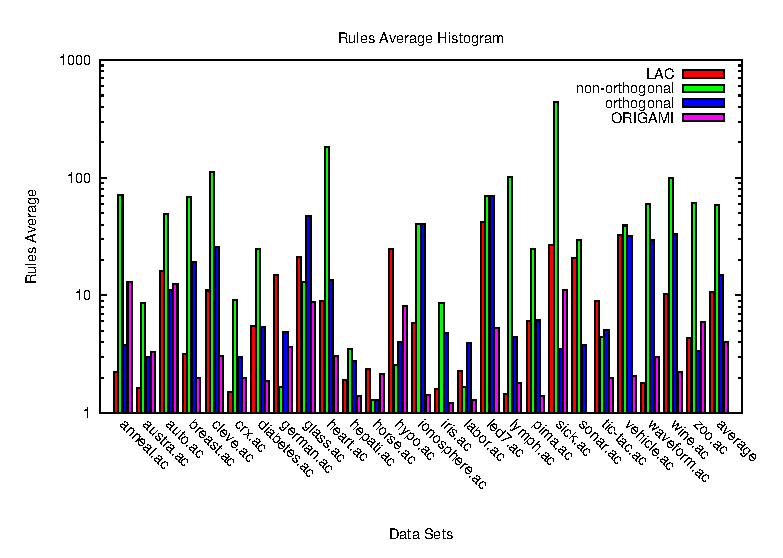
\includegraphics{graphs/histogram_rul.eps}
	\caption{Rules Histogram (best results for each dataset)}
	\label{fig:histogram_acc}
\end{figure}

\begin{figure}[htbp]
	\centering
	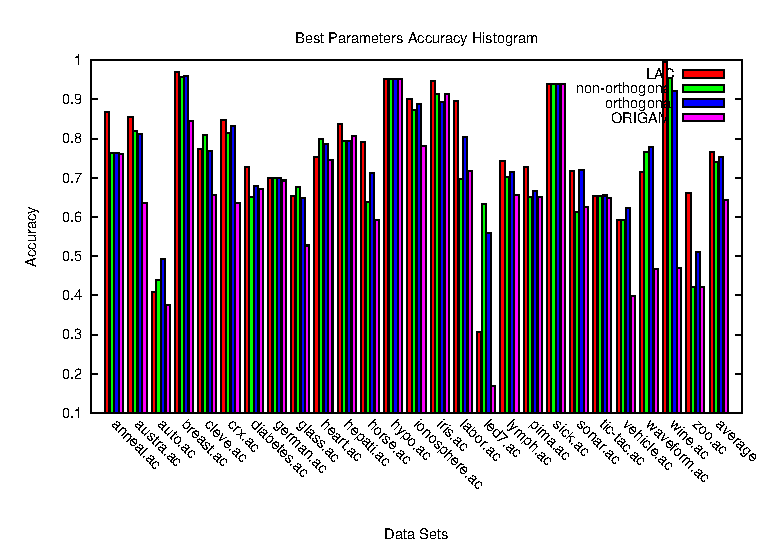
\includegraphics{graphs/bst_histogram_acc.eps}
	\caption{Accuracy Histogram (best average results for all datasets)}
	\label{fig:histogram_acc}
\end{figure}

\section{Compara��o Ortogonal x N�o Ortogonal}

Histogramas de acur�cia, n�mero de padr�es e n�mero de regras. \\
Comparar melhor conjunto de par�metros para cada arquivo e melhor conjunto de par�metros para todos os arquivos juntos.

\section{Compara��o Ortogonal x LAC}

Histogramas de acur�cia, n�mero de padr�es e n�mero de regras. \\
Comparar melhor conjunto de par�metros para cada arquivo e melhor conjunto de par�metros para todos os arquivos juntos.

\section{Compara��o Ortogonal x ORIGAMI}

Histogramas de acur�cia, n�mero de padr�es e n�mero de regras. \\
Comparar melhor conjunto de par�metros para cada arquivo e melhor conjunto de par�metros para todos os arquivos juntos.
